\section{Profile Picture Change}
\label{sec:profilePicChange}
%Why do we explain this?
It can normally be done with a simple uploading of a file and transforming it, into the right size with the build in PHP functions.\\
But in our system it is a bit more complex. Both because we store the images in the Database, so that they can be retrieved on the tablet as well as our PC version. And also because of the before mentioned way we move data around, see section \ref{sec:navigation}.\\
\\
%Why did we make it so complex?
	%Alternative solutions
As again, mentioned in one of the former sections, see section \ref{sec:navigation}, we have made our system this complex in order to minimize the data transferal from the server. This forces us to make some complex solutions to anything that requires big data transferals.\\
As for the database, it is generally bad practice to store images in a database, because of the encoding which is needed to do so. But exactly because we want to be able to use the image both on the tablet as well as on the website, this is actually a good solution. There might have been some alternatives to this, but this is not a part of our project. For more information on this the reader should read the Wasteland project report, which is also a project under the GIRAF project.\\
\\	
%How does the data transfer
As explained at the end of section \ref{sec:navigation}, we have made it so that the upload script is called on submit, from the index files, see listing \ref{lst:largePost}.\\
In order to submit the user must go to the profile page, press the ''Edit'' button underneath the display of the profile picture, they will then be met with a modal window\footnote{A modal window is a sort of pop-up window on a website.} where they are asked to chose a file.

\begin{figure}[htbp]
	\centering
		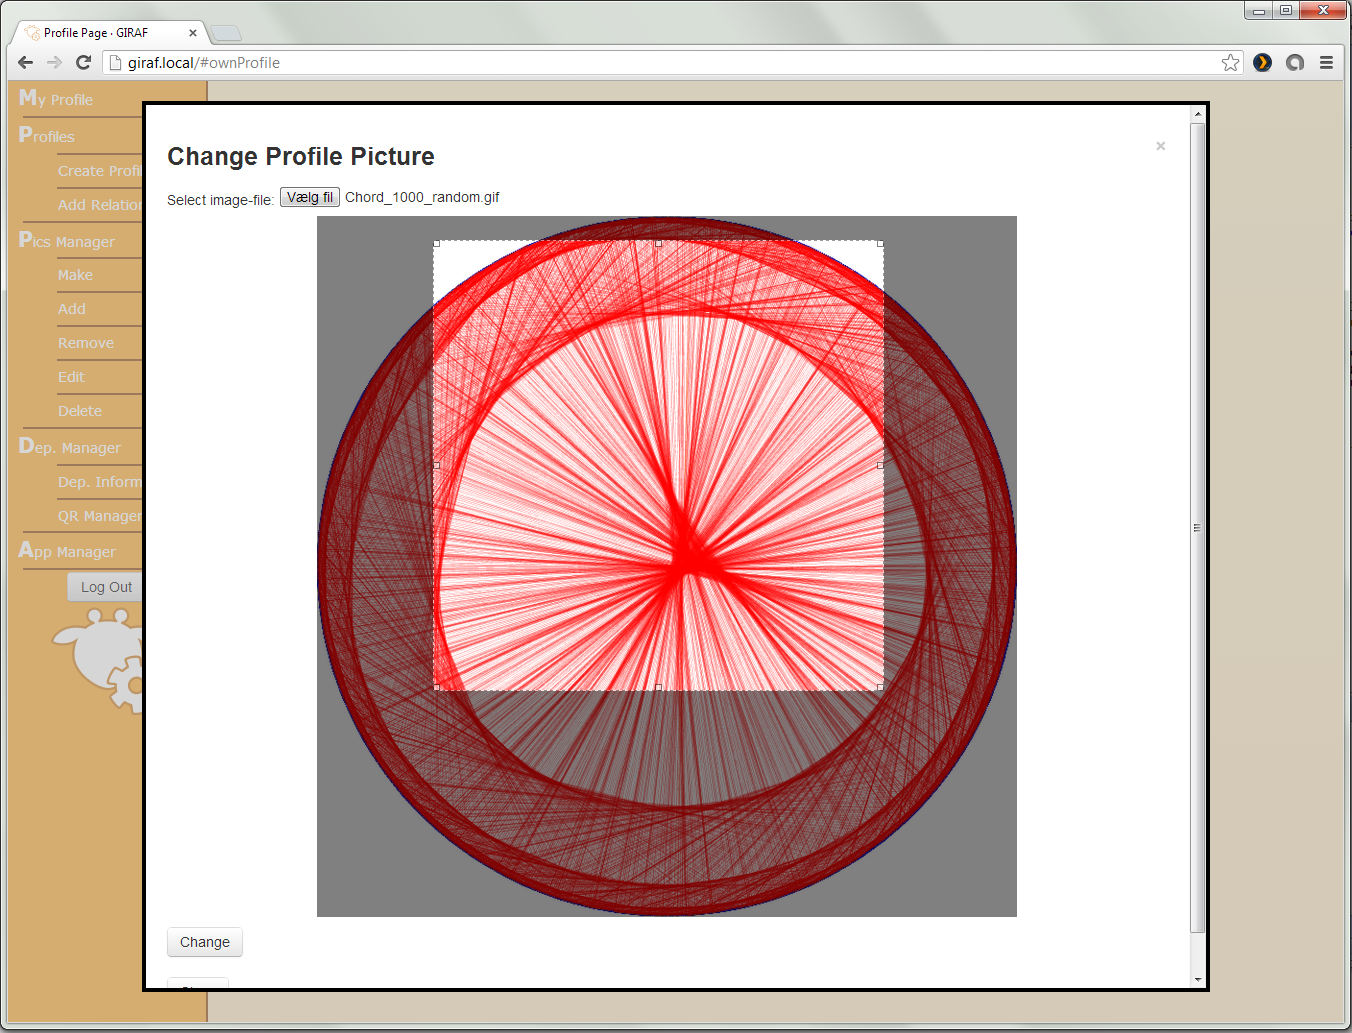
\includegraphics[width=1.0\textwidth]{images/profilePicChange.png}
	\caption{Changing a profile picture}
	\label{fig:profilePicChange}
\end{figure}

When that file is chosen they have to crop the image, as shown on figure \ref{fig:profilePicChange}, and finish by pressing the ''Change'' button.
The cropping here is made with the help of an open source project called imgAreaSelect \citep{imgAreaSelect}.\\
When this is done, the user will be send back to the profile site, with a success or error message and also be able to see the new profile image on the profile.\\
\\
But what the user does not see is that on submit they are actually navigated to our profilePicUpload script, which then navigates them back with the error or success message in the URL.\\
This is the script which handles the encoding and the database query for updating the profile picture.\\
\\
When the profile picture is uploaded the script first checks for any possible upload errors, as well as making sure that the file is actually an image and it was send from our form. This is to prevent security issues.
Then when that is handled, the script will load the image into PHP and will transform it by the help of a specialized cropping tool inspired by a PHP project called SimpleImage \citep{simpleimage}.
\lstset{language=PHP}
\begin{figure}[htbp]
\begin{lstlisting}[firstline=1]
   function resizeCordsColor($width,$height,$x1,$y1,$x2,$y2,$red,$green,$blue) {
      $new_image = imagecreatetruecolor($width, $height);
			$white_image = imagecolorallocate($new_image, $red, $green, $blue); //Change image color to: White (RGB format)
			imagefill($new_image,0,0,$white_image);
      imagecopyresampled($new_image, $this->image, 0, 0, $x1, $y1, $width, $height, $x2-$x1, $y2-$y1);
	  
      $this->image = $new_image;
   }
\end{lstlisting}
\caption{The function used for cropping a profile image.}
\label{lst:croppingProfile}
\end{figure}

The function seen in listing \ref{lst:croppingProfile} is what we use for reshaping the image into a more manageable size. What it does is first to create a new fully white image (L. 2-4), because it is called with the RGB value 255,255,255. Then it proceeds to copy the selected area, which the user selected before onto this white image (L. 5), in a 300 x 300 pixel area, which is the size we decided a profile picture always will be. Finally it stores itself in its own class (L. 7).\\
\\
As for implementing the database query, we have actually designed it and according to the Wasteland API \citep{wastelandApi} it should work. But when we try to update the image it only returns an SQL error in the console. We have asked the Wasteland group why this is so, but they are as clueless as we are. So when the Wasteland group manages to find the error, this feature will be fully implemented.\\
\\
This concludes the explanation of the Profile Picture Changer, if the reader wants to learn more about the Profile Picture Changer the files used for this feature is: \texttt{/include/SimpleImage.php} , \texttt{/assets/js/profileEdit.js} and \texttt{script/profilePicUpload.php} .








%Example of query

%Example of encoding